\subsection{Software}
Für die verschiedenen Versuche und die Umsetzung des Regelkreises müssen Software-Applikationen entwickelt werden. Die Hauptaufgabe besteht in der Berechnung des Regelkreises. Hierfür muss eine HW-Schnittstelle implementiert werden, welche es ermöglicht die Sensorik auszuwerten und die Aktoren anzusteuern. Anschließend müssen die Teilsysteme des Regelkreises berechnet werden. Hierunter fallen die Evaluierung der Sensordaten, die verschiedenen Filter und der letztendliche Regler. Hierbei müssen Echtzeitanforderungen eingehalten werden, welche empirisch im Entwicklungsprozess bestimmt werden.
\begin{figure}[h!]
\centering
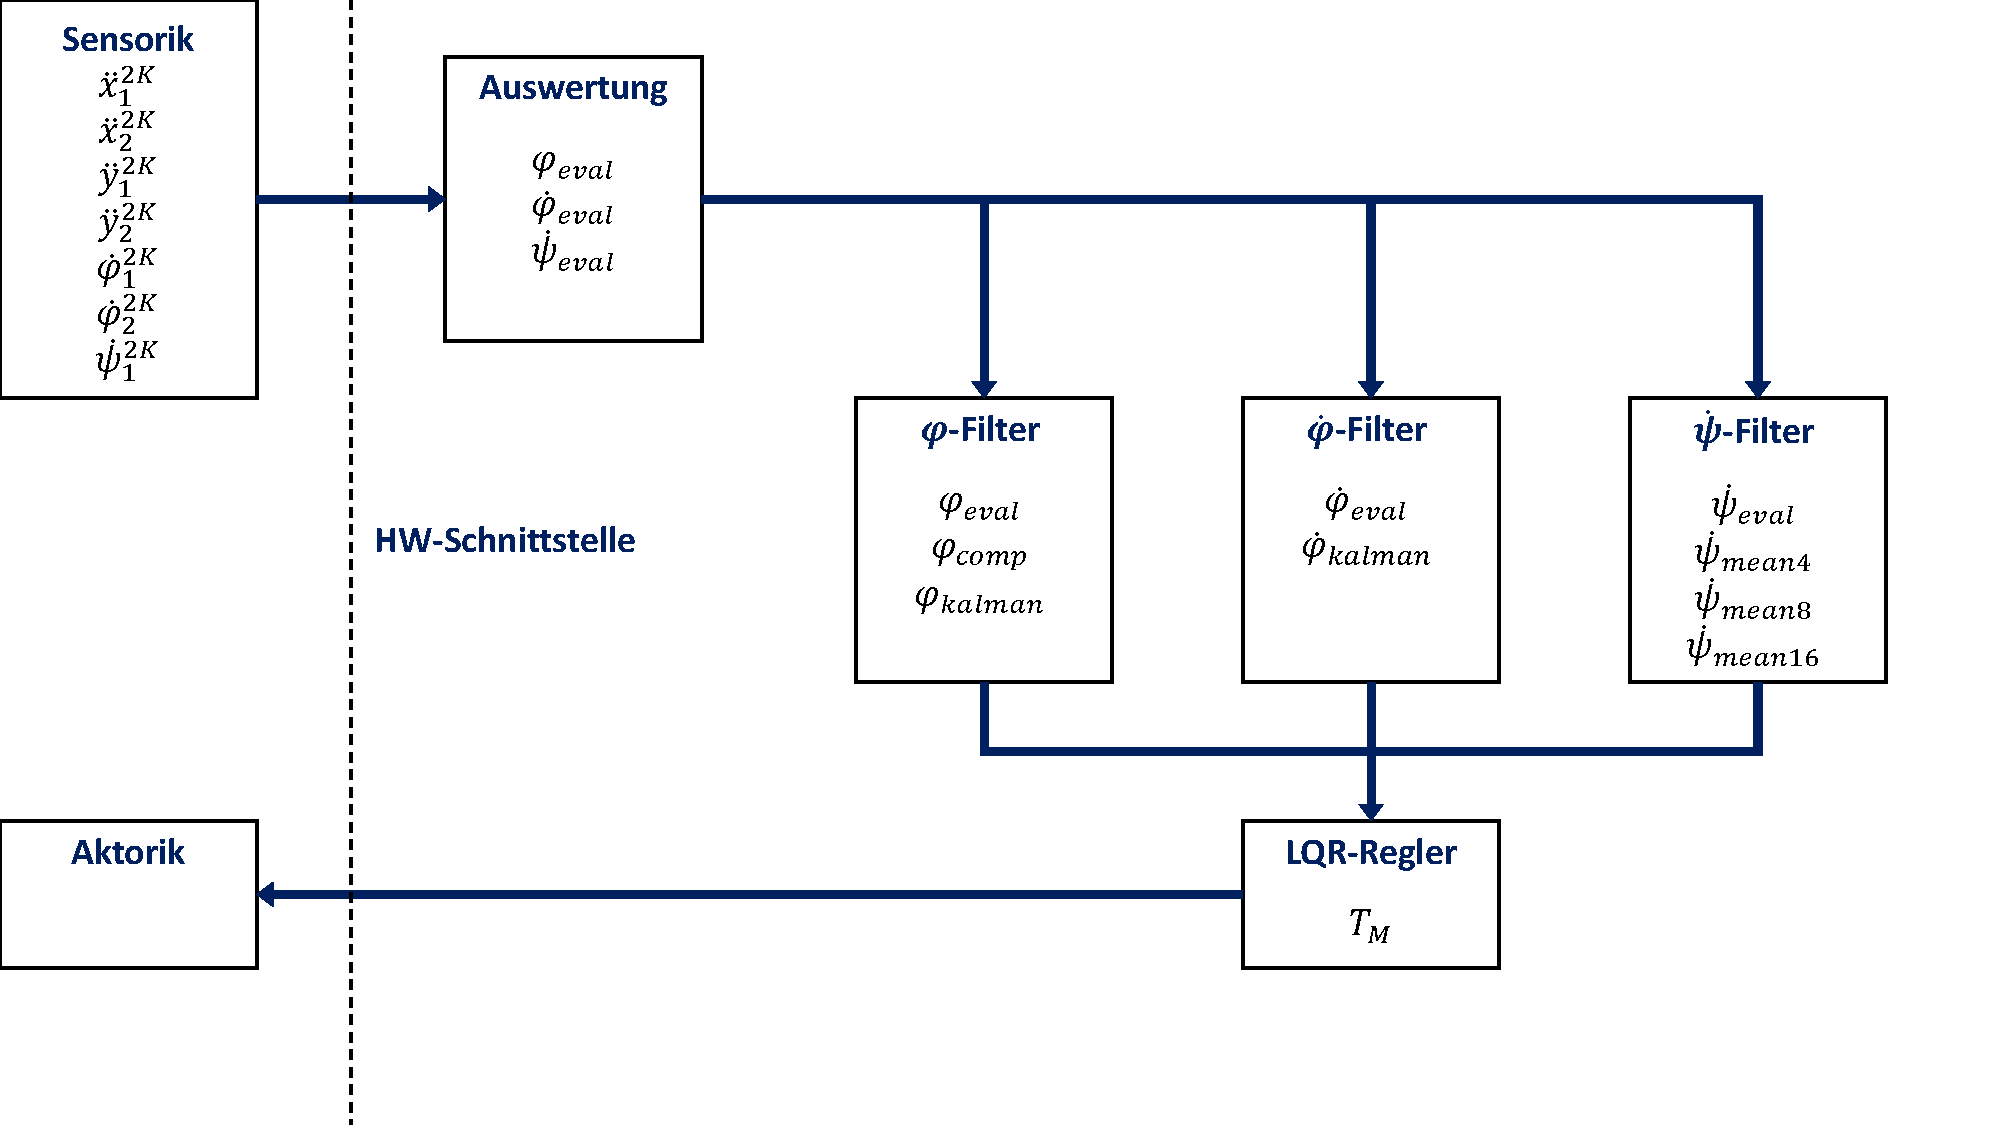
\includegraphics[width=0.6\linewidth]{img/SW_signalfluss_regelkreis}
\caption{Signalfluss Regelkreis, Quelle: eigene Darstellung}
\label{img_signalfluss_regelkreis}
\end{figure}
Abbildung \ref{img_signalfluss_regelkreis} zeigt den Signalfluss des Regelkreises. Für die Durchführung der Versuche müssen die dargestellten Signale an eine MATLAB-Applikation übertragen werden, welche auf dem Host-PC ausgeführt wird. Hierunter fallen die folgenden Daten-Pakete.
\begin{itemize}
\setlength\itemsep{0em}
\item Sensordaten, Rohwerte der Sensoren in 2K-Darstellung
\item $\varphi$-Daten, Werte der Sensorevaluierung, des Komplementär- und Kalman-Filters
\item $\dot{\varphi}$-Daten, Werte der Sensorevaluierung und des Kalman-Filters
\item $\dot{\psi}$-Daten, Werte der Sensorevaluierung und der Mittelwert-Filter
\end{itemize}
Andererseits muss die Anwendung in der Lage sein, Steuerbefehle der MATLAB-Applikation zu empfangen und umzusetzen. Hierunter fallen die folgenden Anweisungen.
\begin{itemize}
\setlength\itemsep{0em}
\item Start- bzw. Stopp-Befehl
\item Auswahl des $\varphi$-Filter
\item Auswahl des $\dot{\varphi}$-Filter
\item Auswahl des $\dot{\psi}$-Filter
\item Setzen des $\varphi$-Offset für die Berechnung des Reglers
\item Setzen des $\dot{\varphi}$-Offset für die Berechnung des Reglers
\item Setzen des $\dot{\psi}$-Offset für die Berechnung des Reglers
\item Setzen eines fixen Motormoment
\end{itemize}
Folglich muss ein Kommunikationsprotokoll implementiert werden um die Verbindung zwischen dem BBB und dem Host-PC herzustellen. Hierbei fällt die Entscheidung auf eine TCP/IP-Verbindung wobei die BBB-Anwendung als Server agiert. Die Gründe für das gewählte Protokoll sind einerseits die komfortable Implementierung auf beiden Seiten, andererseits die Sicherung der fehlerfreien Datenübertragung.

\subsection{Allgemeiner Softwareentwurf}
Die oben genannten Aufgaben werden auf zwei logische Komponenten verteilt, welche als separate Tasks ausgeführt werden. Hierbei übernimmt die Regelungskomponente die Berechnung des Regelkreises und die Bereitstellungen der Daten. Die Kommunikationskomponente betreibt den TCP/IP-Server um Daten an MATLAB zu senden bzw. zu empfangen. Zusätzlich muss ein dritter Task realisiert werden, welcher für die Zeitgebung verantwortlich ist. 

\subsubsection{Kommunikation zwischen den Komponenten}
Der Datenaustausch zwischen den Tasks wird mit Hilfe von Nachrichten implementiert, welche sich aus Steuerinformationen über Typ bzw. Inhalt und einem Datenpaket zusammensetzen. Die Grund für die Entscheidung Nachrichten für die Datenübertragung zu verwendet ist einerseits, dass nur kleine Datenpakete übermittelt werden müssen, andererseits können die Nachrichten als TCP/IP-Paket wiederverwendet werden. Somit besteht die Aufgabe der Kommunikationseinheit in der Weiterleitung von Nachrichten mit Regeldaten an MATLAB bzw. der Weiterleitung von Nachrichten mit Befehlen an den Proxy. Diese werden von einem zentralen Proxy erzeugt und zugestellt. Da die Empfänger der verschiedenen Nachrichtentypen vor Laufzeit bekannt sind ist keine dynamische Registrierung der Komponenten erforderlich.

\begin{figure}[!h]
\centering
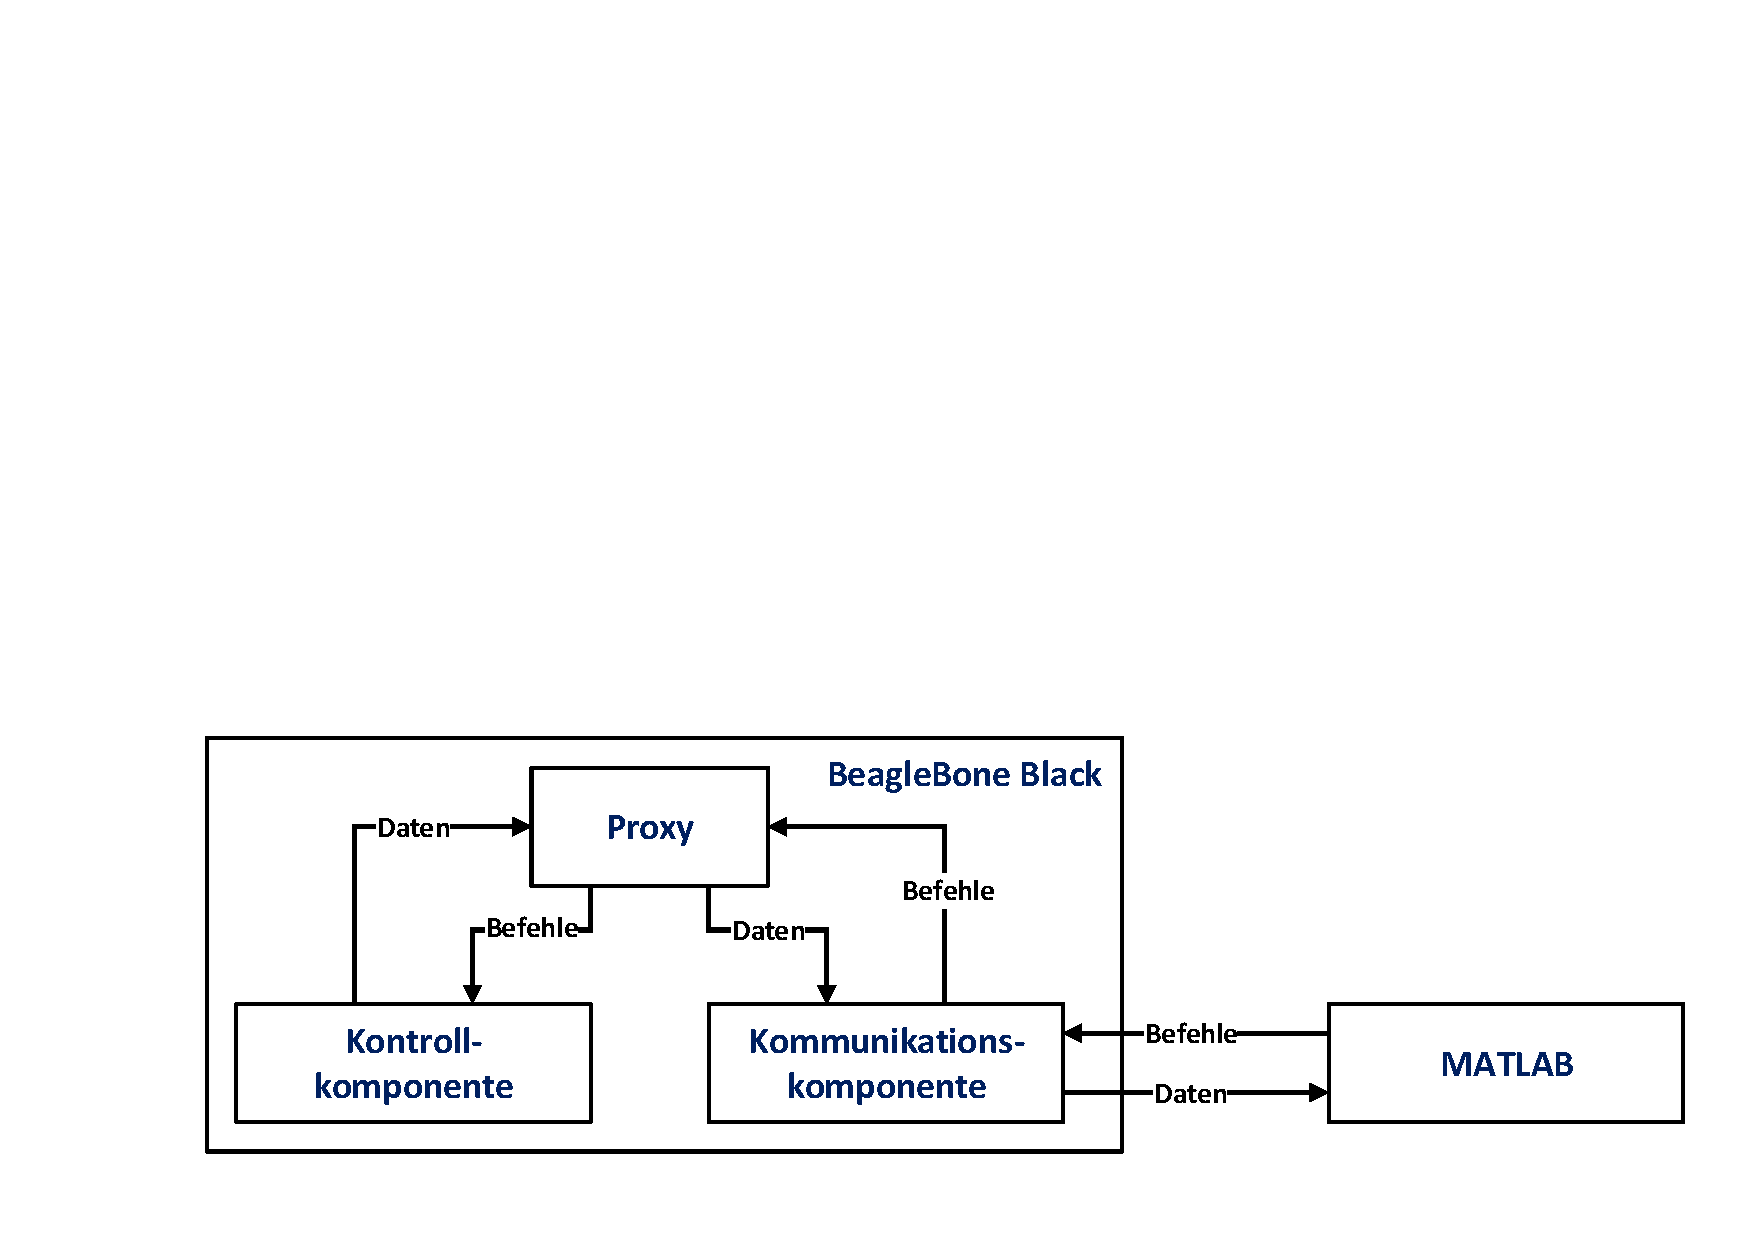
\includegraphics[width=0.8\linewidth, trim={0cm 0cm 2cm 9cm},clip]{img/SW_kommunikation}
\caption{SW-Kommunikation, Quelle: eigene Darstellung}
\label{img_kommunikation_sw}
\end{figure}

Nach Abbildung \ref{img_kommunikation_sw} werden Nachrichten für die Übertragung von Daten aus dem Regelkreis und für die Zustellung von Befehlen verwendet. Folglich setzt sich der Header aus dem Nachrichtentyp und dem Befehl bzw. Datentyp zusammen. Die Größe des Datenfeldes ist fix und wird nach dem größten Signalpaket ausgerichtet. Dadurch vereinfacht sich die Übertragung der Nachrichten über den TCP/IP-Stream.

\begin{lstlisting}
class CMessage
{
public:
	struct CHeader
	{
	EMessageType mType;
	ECommand mCommand;
	EDataType mDataTyp;
	}
	...
private:
	CHeader mHeader;
	static constexpr Int32 sSize = 20;
	UInt8 mData[sSize];
};
\end{lstlisting}

Um Nachrichten zu empfangen verfügen die Komponenten über Eingangspuffer, welche als Queues implementiert werden. Das Grundgerüst der Komponenten wird in einer abstrakten Basisklasse festgelegt, welche rein virtuelle Methoden zur Initialisierung und Ausführung deklariert. Die \textit{dispatch}-Methode ist für die Verarbeitung von Nachrichten zuständig.

\begin{lstlisting}
class AComponentBase
{
public:
	virtual void init() = 0;
	virtual void run() = 0;
protected:
	TQueue<Config::QueueSize> mQueue;
}
\end{lstlisting}

Die Erzeugung und Zustellung von Nachrichten übernimmt ein Proxy, welcher Methoden für die verschiedenen Ereignisse zur Verfügung stellt. Dadurch wird die Kommunikationsstruktur gekapselt, wodurch eine übersichtliche Applikation entsteht. Der Proxy kennt die Eingangsqueues der Komponenten und reicht die Nachrichten nach Typ an die Empfänger weiter.

\newpage
\begin{lstlisting}
class CProxy
{
public:
	bool clientDisconnect(bool waitForever);
	bool transmitSensorData(const CSensorData& data, bool waitForever);
	bool transmitPhi(const CPhi& data, bool waitForever);
	bool transmitPhi__d(const CPhi__d& data, bool waitForever);
	bool transmitPsi__d(const CPsi__d& data, bool waitForever);
	bool timerTick(bool waitForever);
	bool routeMATLABMessage(bool waitForever);
	...
private:
	TQueue& mControlQueue;
	TQueue& mCommQueue;
}
\end{lstlisting}

\subsubsection{Aufbau der Regelungskomponente}
Die Aufgaben der Regelungskomponente bestehen einerseits in der Interaktion mit der HW und der Berechnung des Regelkreises. Diese Teilsysteme werden als Klassen implementiert, welche Methoden bereitstellen um die Sensorwerte auszulesen, die Motoren zu steuern und die Filterwerte bzw. den Regler zu berechnen. Zusätzlich gehört der Timer-Task zu der Regelungskomponente und wird als eigenständiger Thread ausgeführt. 

\begin{figure}[!h]
\centering
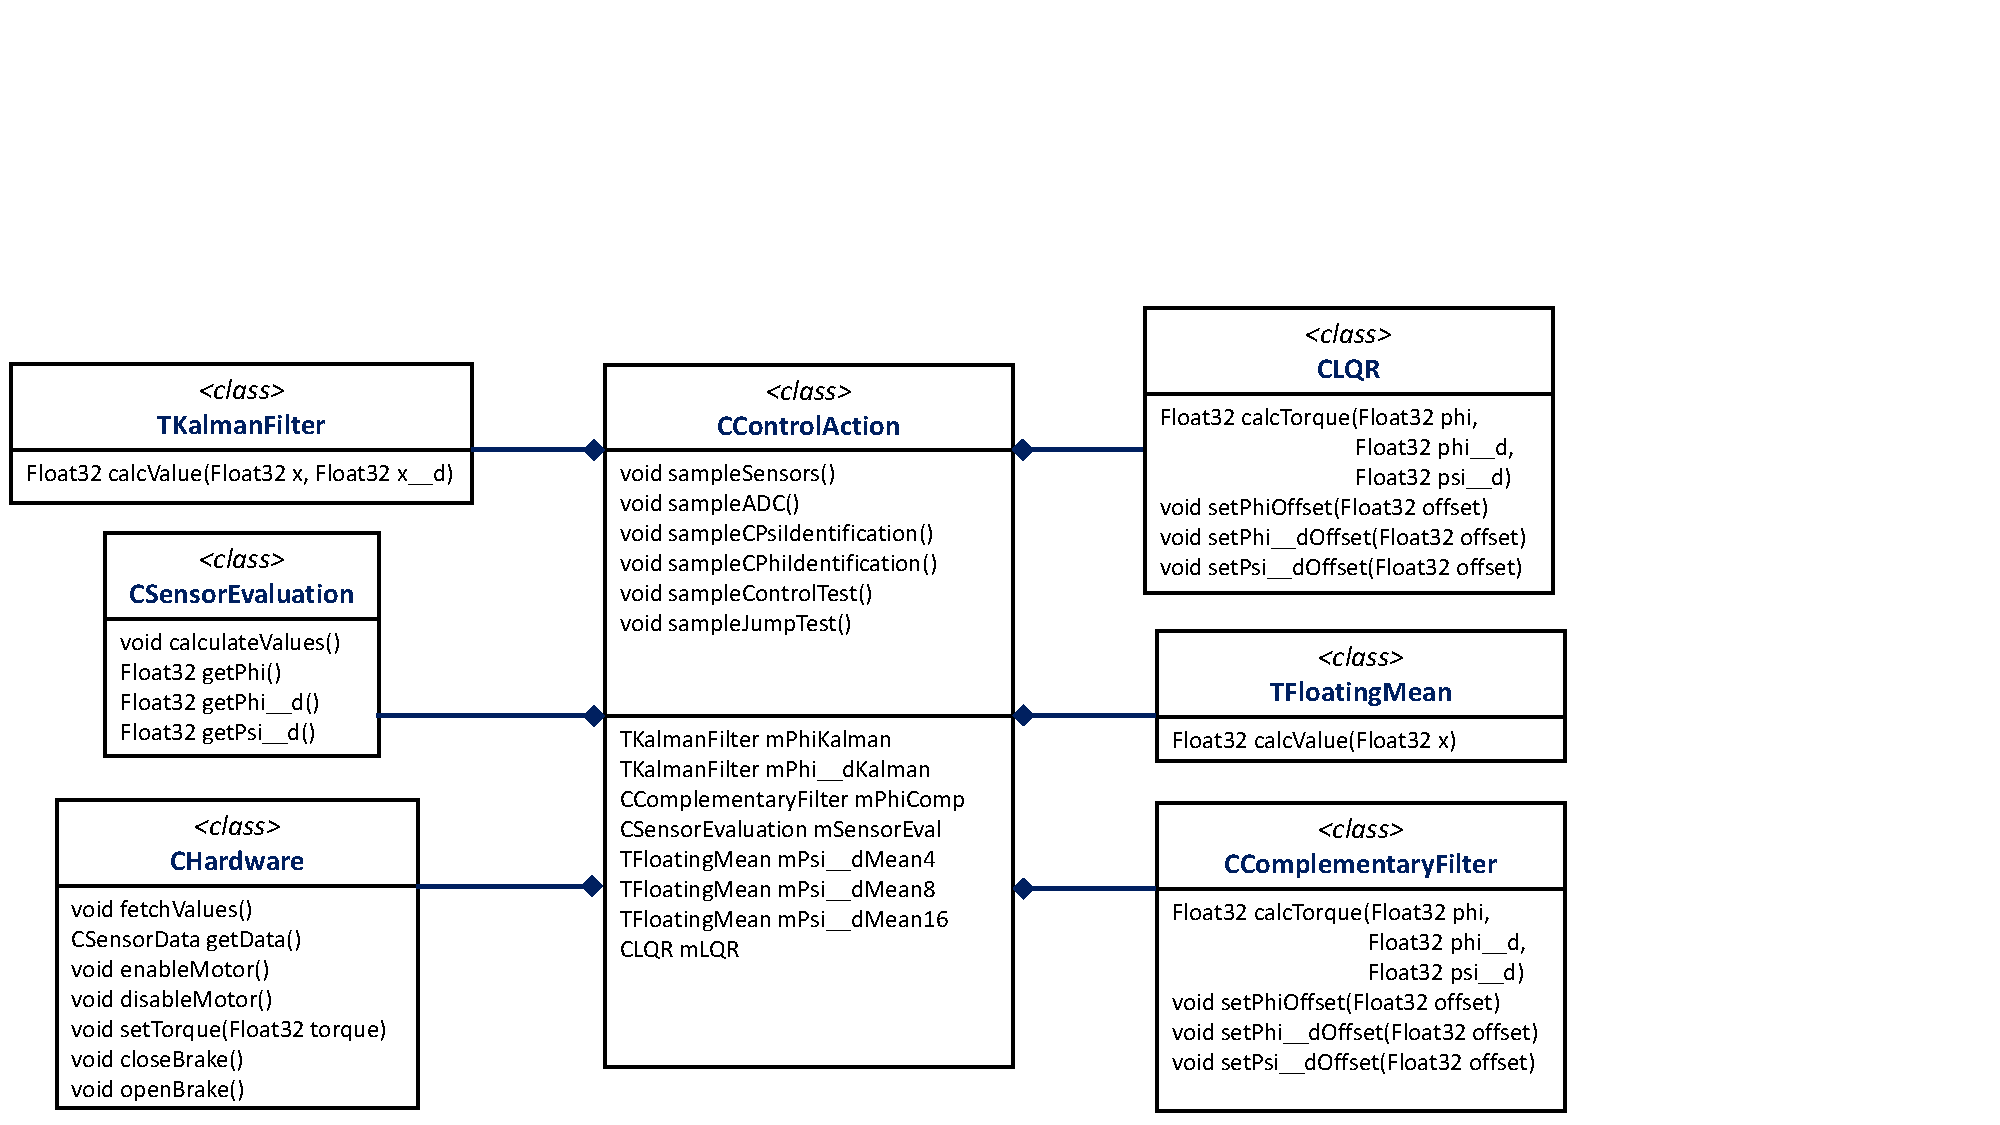
\includegraphics[width=\linewidth, trim={0cm 0cm 7cm 5cm}, clip]{img/SW_KontrollKlassen}
\caption{Klassendiagramm Regelkreis, Quelle: eigene Darstellung}
\end{figure}

Für die verschiedenen Versuche ist eine zusätzliche Kontrolllogik erforderlich, welche in Form eines Zustandsautomaten implementiert wird. Die FSM verarbeitet die empfangenen Nachrichten und passt den aktuellen Zustand und somit das Verhalten entsprechend an. Auf der obersten Schicht verfügt das Statechart über den Zustand \textit{STANDBY} und Zustände um die verschiedenen Versuche durchzuführen. Dadurch kann dieselbe Applikation flexibel eingesetzt und während des Entwicklungsprozesses erweitert werden. Die letztendlichen Aufgaben der Komponente, wie z.B. die Auswertung der Sensorik und Signalverarbeitung, werden in der Klasse \textit{CControlAction} gekapselt um eine klare Trennung von Kontroll- und Signalfluss zu gewährleisten.

\begin{figure}[!h]
\centering
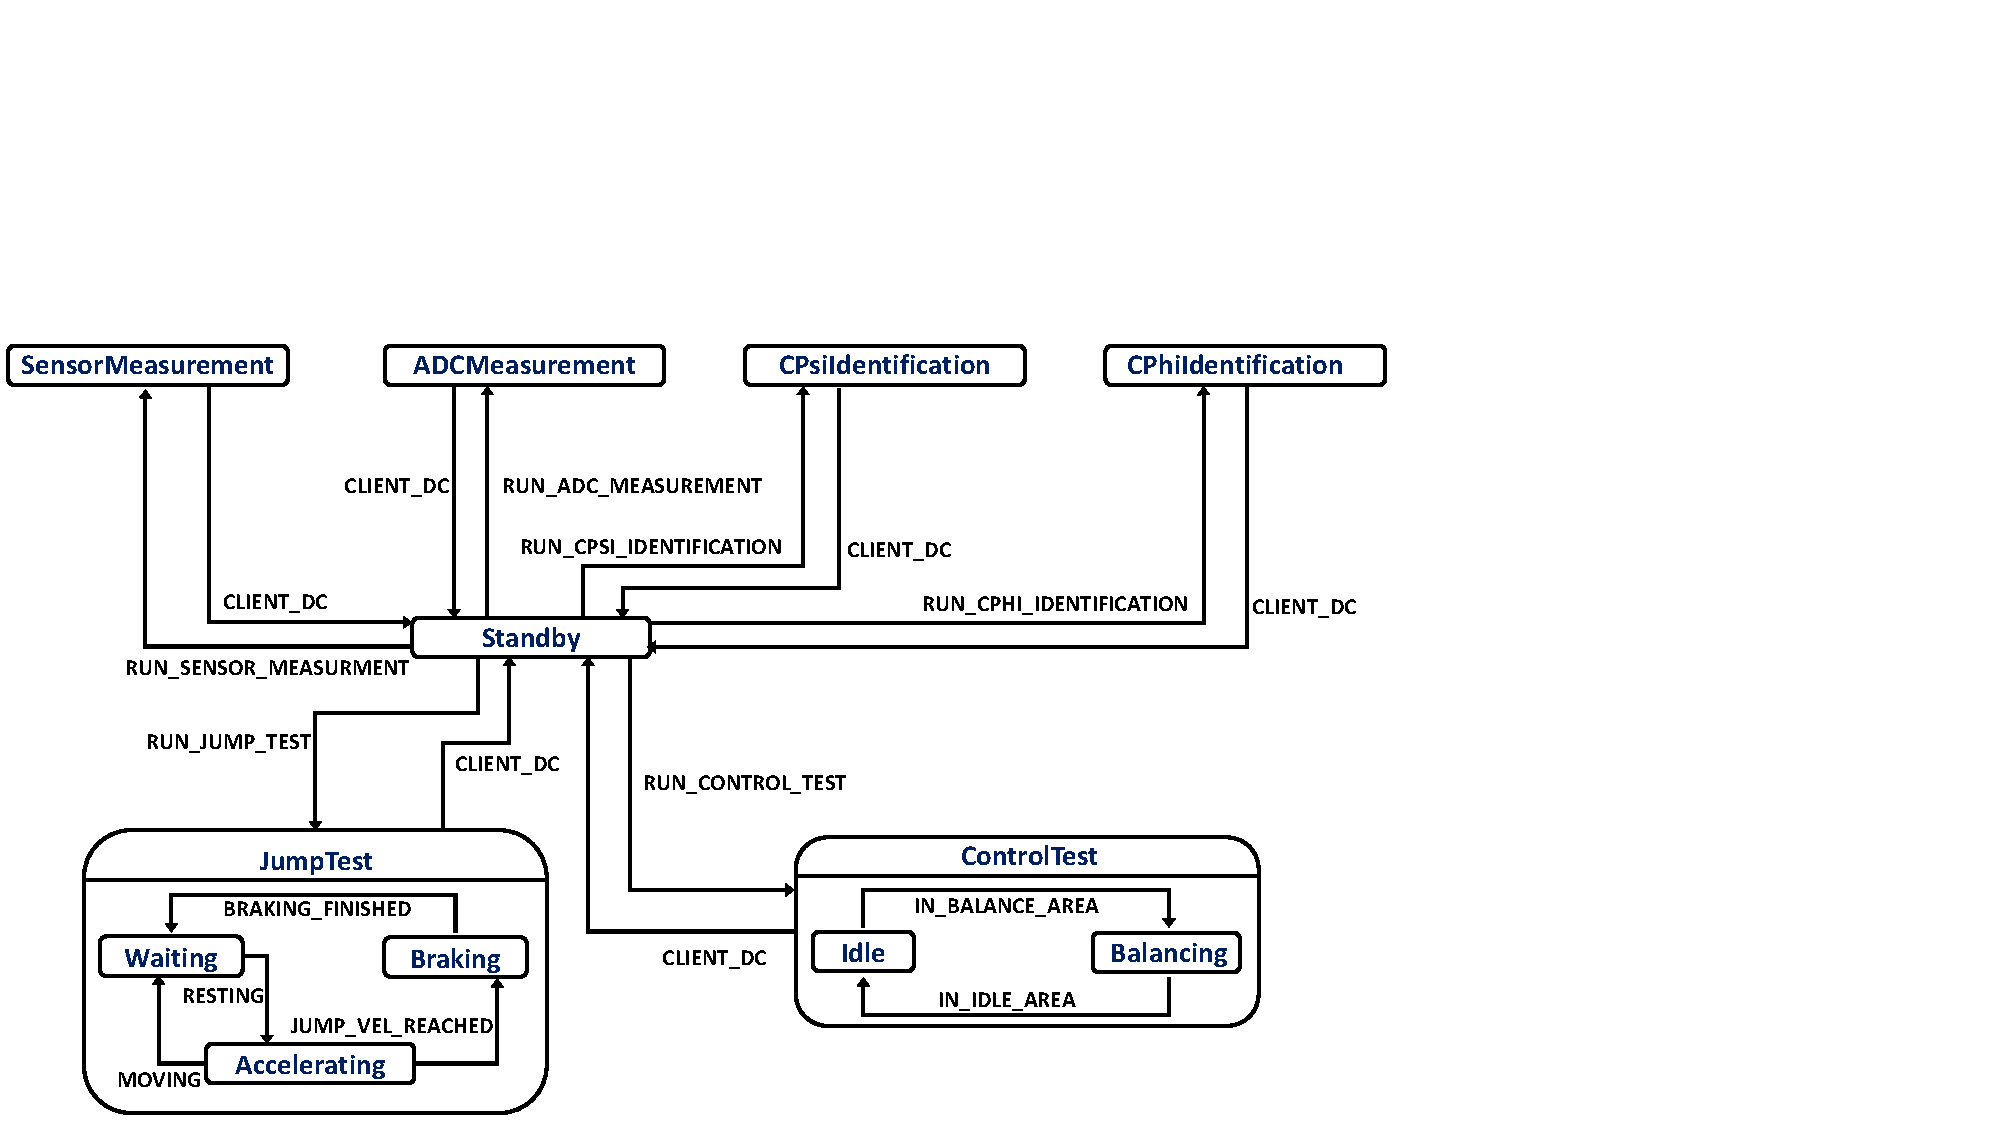
\includegraphics[width=1\linewidth, trim={0cm 0cm 10cm 5.5cm}, clip]{img/SW_KontrollFSM}
\caption{Kontroll-FSM, Quelle: eigene Darstellung}
\end{figure}


Bei Betreten der Versuch-Zustände wird der Softtimer gestartet, welcher zyklisch Timer-Events an die Regelungskomponente sendet. Bei Erhalten einer solchen Nachricht führt die FSM die, dem aktuellen Zustand entsprechende, Logik aus. 
Die ersten drei Versuche sind aus Sicht des Kontrollflusses identisch, aus Gründen der Einheitlichkeit werden dennoch drei explizite Zustände implementiert. In diesen Zuständen werden bei Eintreffen eines Timer-Events die aktuellen Sensorwerte abgefragt und and die MATLAB-Applikation gesendet. Für die Versuche 4 und 5 müssen die Sensorauswertung und die Filter implementiert werden. Deren Ausgangswerte werden wiederum zyklisch berechnet und mit Hilfe des Proxys an MATLAB übertragen. Versuch 6 besteht in der Umsetzung des Reglers. Der entsprechende Zustand muss einerseits den vollständigen Regelkreis berechnen, als auch die Filter- und Reglerwerte an MATLAB übertragen. Zusätzlich muss der Zustand die Befehle zur Auswahl der Filter und zum Setzen der Offsets annehmen und umsetzen.

\subsubsection{Aufbau der Kommunikationskomponente}
Die Hauptaufgabe der Kommunikationseinheit besteht in dem Betrieb des TCP/IP-Server und der Weiterleitung von Nachrichten. Der Server wird in Form einer Klasse implementiert, welche Methode zum Empfangen und Versendet von Nachrichten bereitstellt. 

\begin{lstlisting}
class CServer
{
	public:
	void init();
	void waitForConnection();
	bool transmitMessage(CMessage& msg, bool waitForever);
	bool receiveMessage(CMessage& msg, bool waitForever);
	...
	private:
		Int32 mSocketFD;
		Int32 mConnectionFD;
}
\end{lstlisting}

Hierfür wird ein zweiter Thread gestartet, welcher auf Nachrichten der MATLAB-Anwendung wartet und diese an den Proxy weiterleitet. Die Kontrolllogik der Komponente wird ebenfalls in Form einer Zustandsmaschine implementiert. Hierbei wird lediglich zwischen den Zuständen \textit{STANDBY} und \textit{RUNNING} unterschieden. Im Ausgangszustand wartet die Komponente auf die Verbindungsanfrage eines Client, welcher die MATLAB-Anwendung ist. Der Haupt-Thread der Komponente wartet auf eingehende Ereignisse und verarbeitet diese. Der zweite Thread wartet zuerst auf die Verbindungsanfrage des Client, diese signalisiert er mittels einer Nachricht. Daraufhin wechselt die Komponente in den \textit{RUNNING}-Zustand, in welchem empfangene Nachrichten mit Regelungsdaten an MATLAB weitergeleitet werden. Der zweite Thread wartet nun auf eingehende TCP/IP-Daten von MATLAB. Sowohl beim senden als auch empfangen von Daten kann ein Verbindungsabbruch des Clients erkannt werden. In diesem Fall wechselt die Komponente in den \textit{STANDBY}-Zustand und der zweite Thread wartet auf eine neue Verbindungsanfrage.